\documentclass{HZNUMCM}
\usepackage{graphicx}
\usepackage{hyperref}
\usepackage{subcaption}
\definecolor{customcolor}{HTML}{325AA0}

\setControlNumber{888888}
\setContestType{MCM}
\setProblemLetter{A}
\setPaperTitle{Our Article}

%summary
\setSummary{ sumary sumary sumary sumary sumary sumary sumary sumary sumary sumary sumary sumary sumary sumary sumary sumary sumary sumary sumary sumary sumary sumary sumary sumary sumary sumary sumary sumary sumary sumary sumary sumary sumary sumary sumary sumary sumary sumary sumary sumary sumary sumary sumary sumary sumary sumary sumary sumary sumary sumary sumary sumary sumary sumary sumary sumary sumary sumary sumary sumary sumary sumary sumary sumary sumary sumary sumary sumary sumary sumary sumary sumary sumary sumary sumary sumary sumary sumary sumary sumary sumary sumary sumary sumary sumary sumary sumary sumary sumary sumary sumary sumary sumary sumary sumary sumary sumary sumary sumary sumary sumary sumary sumary sumary sumary sumary sumary sumary sumary sumary sumary sumary sumary sumary sumary sumary sumary sumary sumary sumary sumary sumary sumary sumary sumary sumary sumary sumary sumary sumary sumary sumary sumary sumary sumary sumary sumary sumary sumary sumary sumary sumary sumary sumary sumary sumary sumary sumary sumary sumary sumary sumary sumary sumary sumary sumary sumary sumary sumary sumary sumary sumary sumary sumary sumary sumary sumary sumary sumary sumary sumary sumary sumary sumary sumary sumary sumary sumary sumary sumary sumary sumary sumary sumary sumary sumary sumary sumary sumary sumary sumary sumary sumary sumary sumary sumary sumary sumary sumary sumary sumary sumary sumary sumary sumary sumary sumary sumary sumary sumary sumary sumary sumary sumary sumary sumary sumary sumary sumary sumary sumary sumary sumary sumary sumary sumary sumary sumary sumary sumary sumary sumary sumary sumary sumary sumary sumary sumary sumary sumary sumary sumary sumary sumary sumary sumary sumary sumary sumary sumary sumary sumary sumary sumary sumary sumary sumary sumary sumary sumary sumary sumary sumary sumary sumary sumary sumary sumary sumary sumary sumary sumary sumary sumary sumary sumary sumary sumary sumary sumary sumary sumary sumary sumary sumary sumary sumary sumary sumary sumary sumary sumary sumary sumary sumary sumary sumary sumary sumary sumary sumary sumary sumary sumary sumary sumary sumary sumary sumary sumary sumary sumary sumary sumary sumary sumary sumary sumary sumary}

%begin
\begin{document}
\showSummarySheet
\showContents

  \section{Introduction}
    \subsection{Background}
    \subsection{Problem Analysis}
    \subsection{Our Work}
    \begin{itemize}
      \item work1
      \item work2
      \item work3
    \end{itemize}

  \section{Assumptions and Notation}
    \subsection{Assumptions and Explanation}
    \subsection{Notations}

  \section{Models}

  \section{Application of the Models}

  \section{Sensitivity Analysis}

  \section{Evaluation of the Model}
    \subsection{Strengths}
    \subsection{Weaknesses}

  \section{Conclusion}

  % % figure
  % \begin{figure}[ht]
  %   \centering
  %   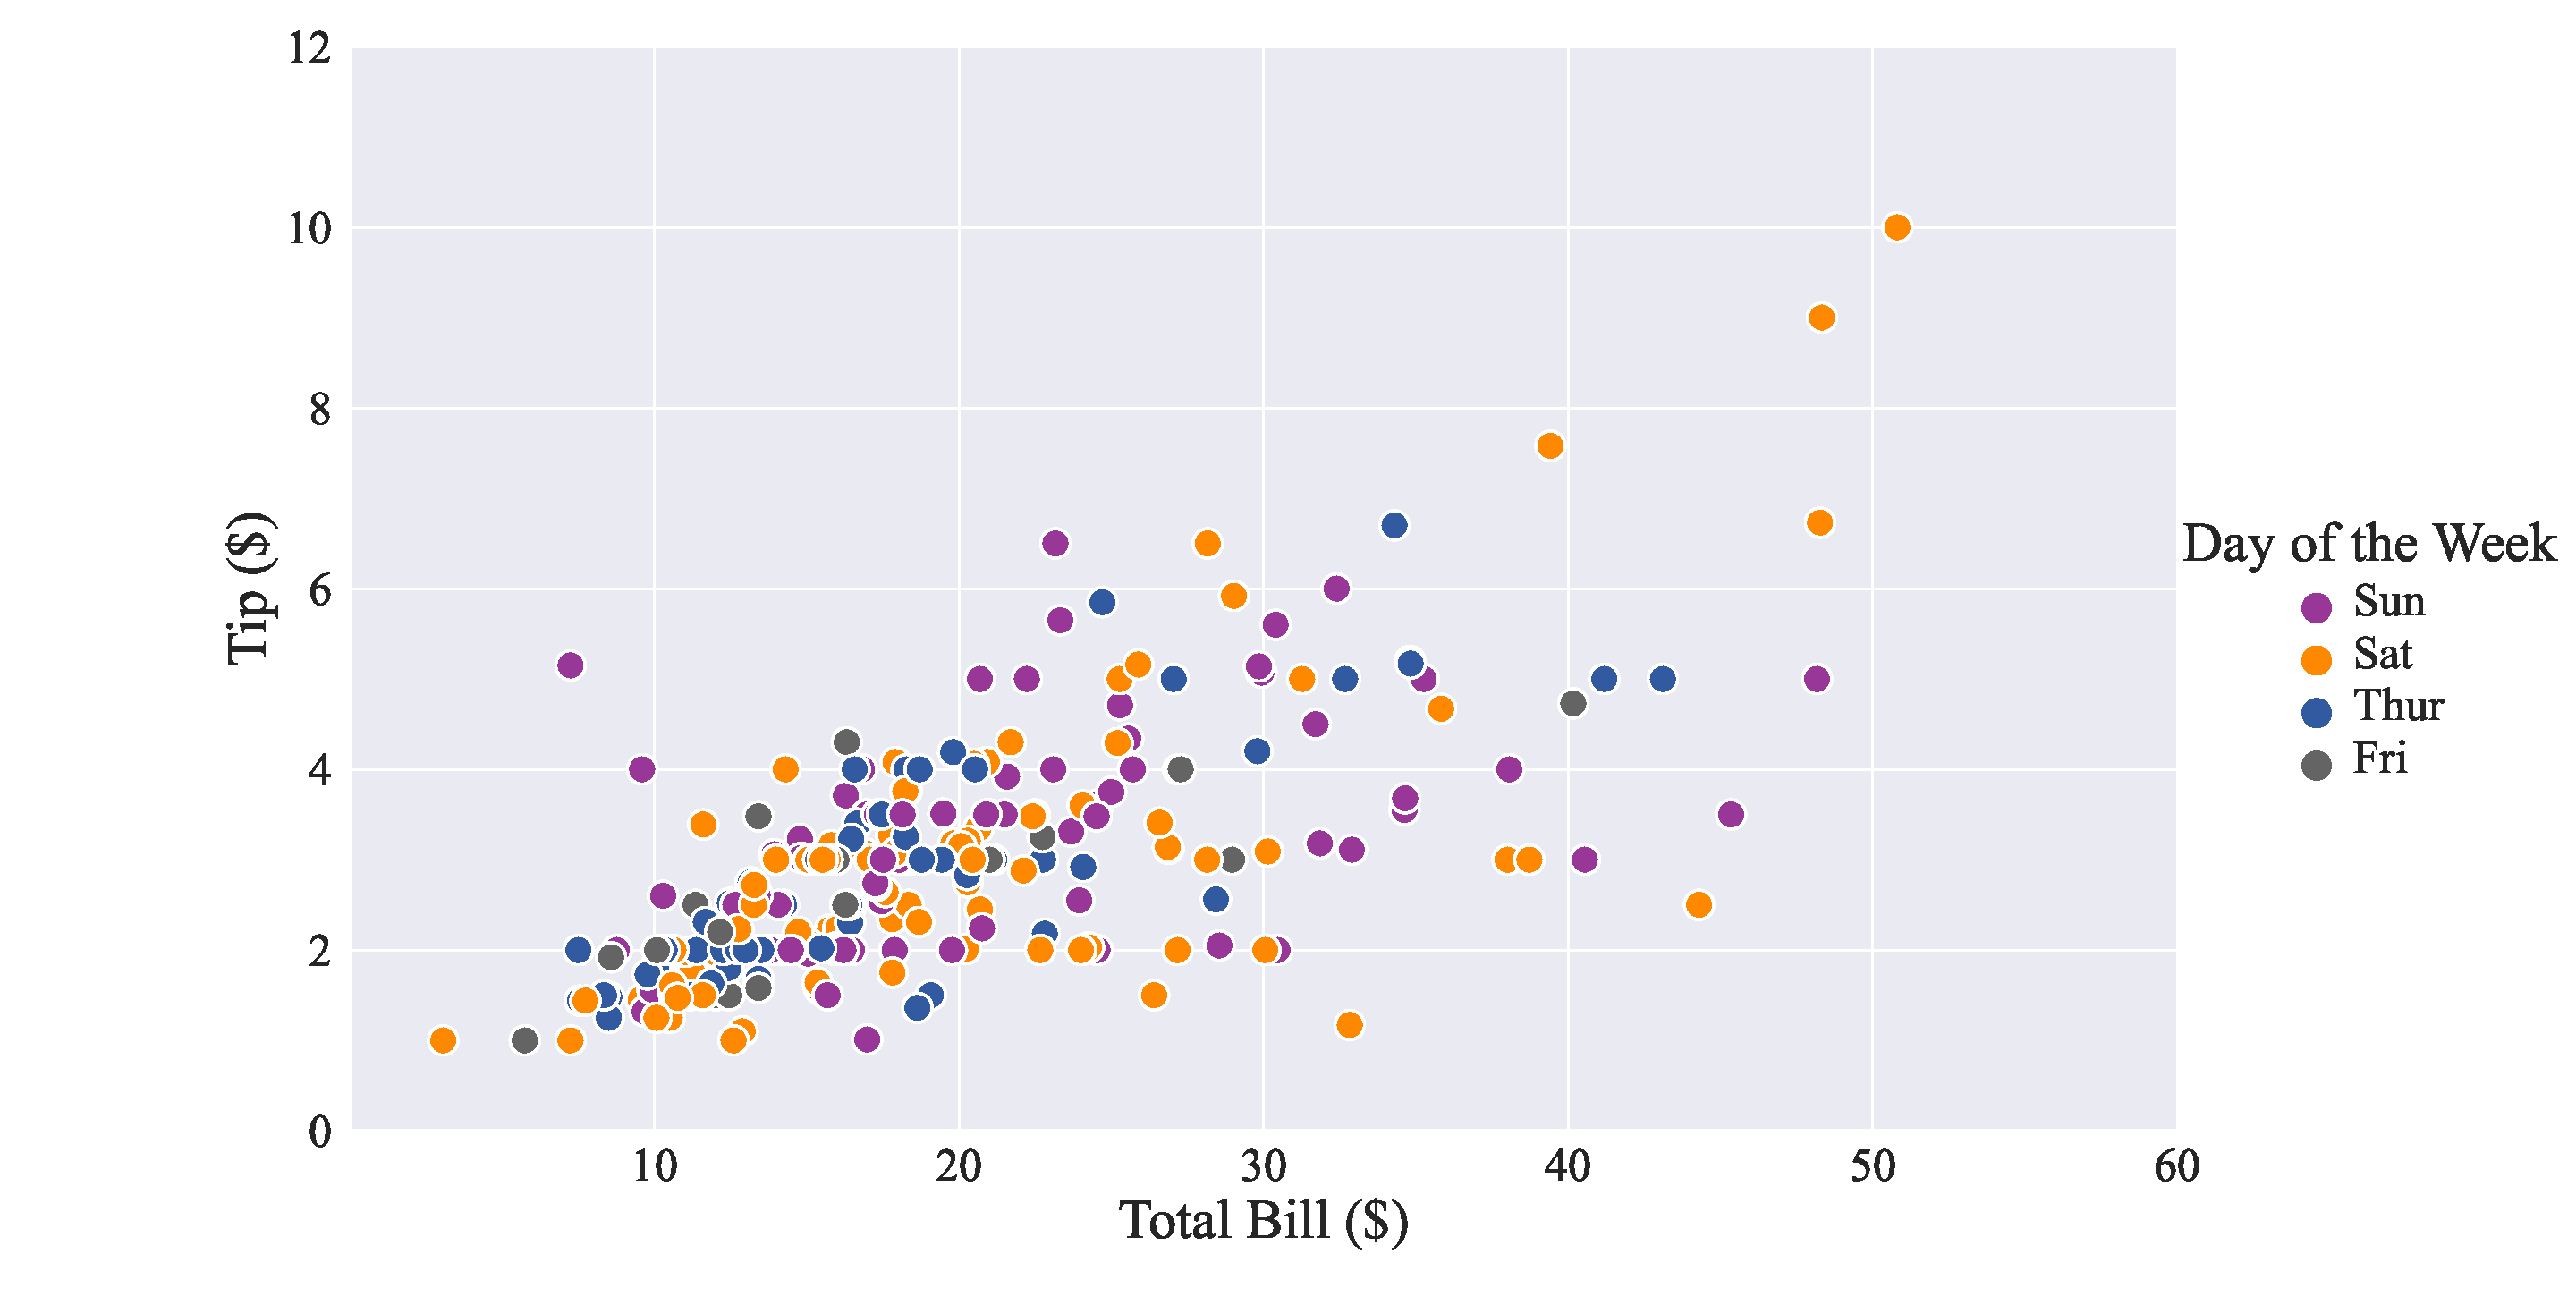
\includegraphics[width=\linewidth]{images/scatter.pdf} % 替换为你的第一张图片路径
  %   \caption{the scatter}
  %   \label{fig:image1}
  % \end{figure}

  % \begin{figure}[ht]
  %     \centering
  %     \begin{minipage}[b]{0.45\linewidth}
  %         \centering
  %         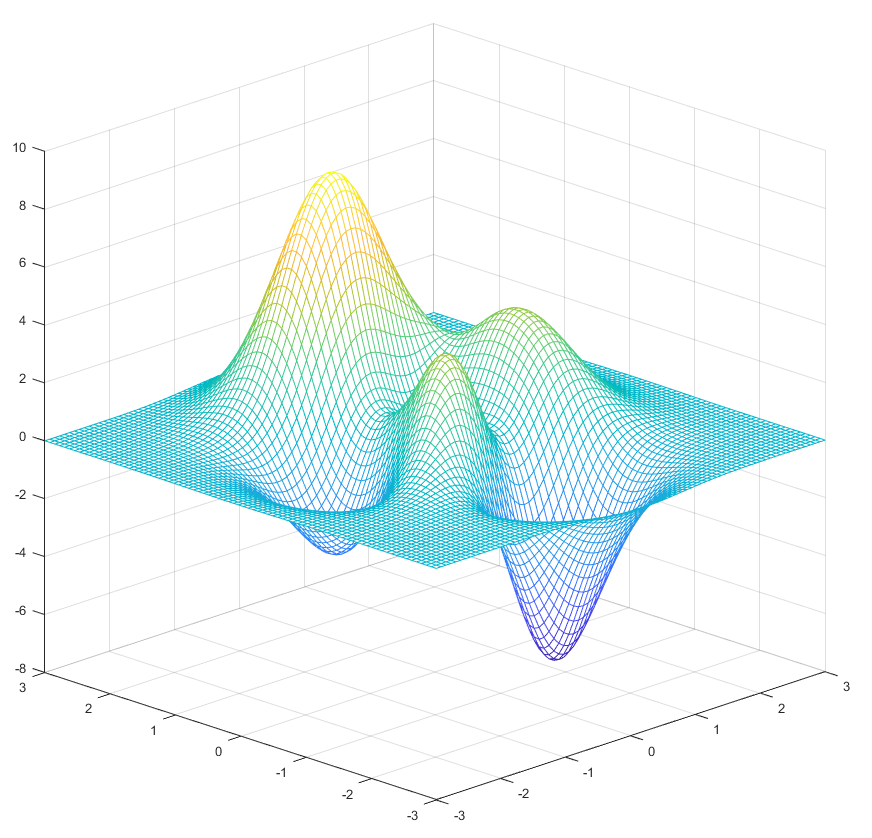
\includegraphics[height=5cm, keepaspectratio]{images/peaks.png} % 替换为你的第一张图片路径
  %         \caption{First Image}
  %         \label{fig:image2}
  %     \end{minipage}
  %     \hspace{0.05\linewidth}
  %     \begin{minipage}[b]{0.45\linewidth}
  %         \centering
  %         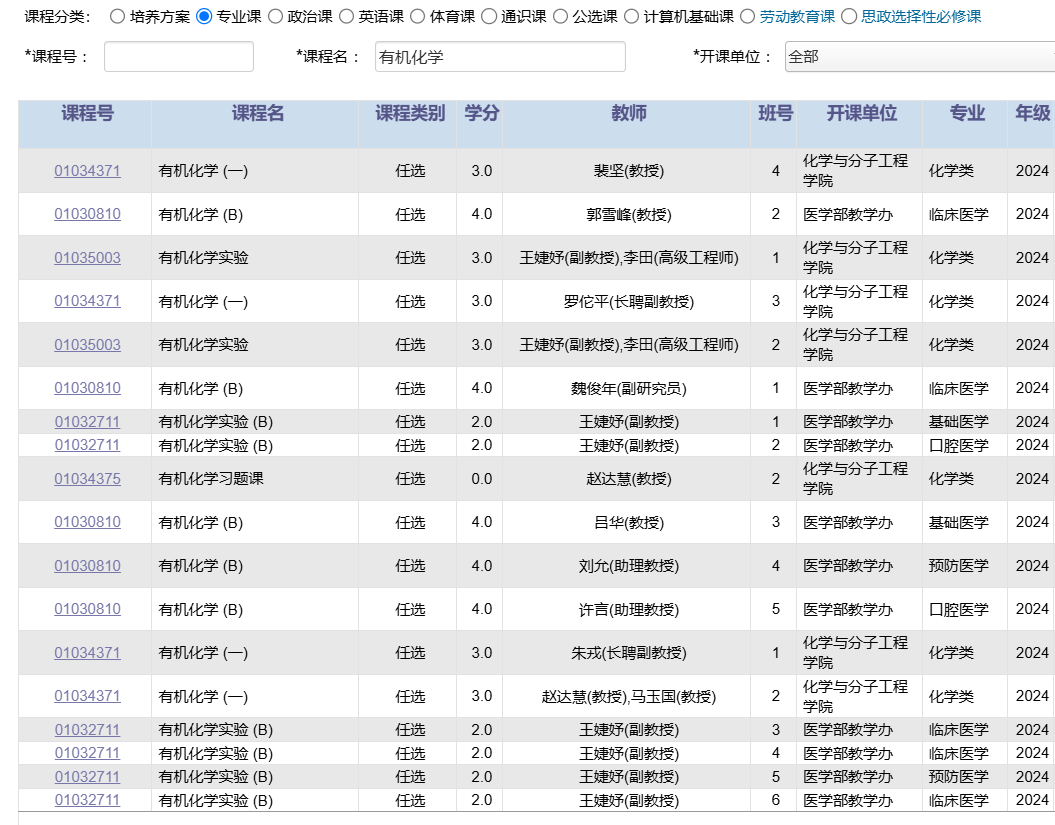
\includegraphics[height=5cm, keepaspectratio]{images/courses.png} % 替换为你的第二张图片路径
  %         \caption{Second Image}
  %         \label{fig:image3}
  %     \end{minipage}
  % \end{figure}

  %%citation
  % as \figurename~\ref{fig:image1} shows,this is a picture.
  % ...\cite{example1}
  % 123123123\cite{rosenow1983drought}

  % % table
  % \begin{table}[h]
  %   \centering
  %   \caption{An example of a three-line table.}
  %   \begin{tabular}{lccc}
  %     \toprule
  %     \rowcolor{customcolor!50} % 设置背景颜色
  %     Column 1 & Column 2 & Column 3 & Column 4 \\
  %     \midrule
  %     Data 1 & Data 2 & Data 3 & Data 4 \\
  %     Data 4 & Data 5 & Data 6 & Data 8 \\
  %     \bottomrule
  %   \end{tabular}
  %   \label{tab:example}
  % \end{table}

  \addcontentsline{toc}{section}{References}
  \bibliographystyle{unsrt}%{brief}%{alpha}%{unsrt}
  \bibliography{article_file}

\end{document}